%%==================================================
%% chapter04.tex for BIT Master Thesis
%% modified by 朱杰
%%==================================================
\chapter{基于稳定标签传播的重叠社区发现算法}
在验证了上一章所提稳定策略在 LPA 算法上的有效性的基础上,将此稳定策略运用到 COPRA 算法中,以验证其在重叠社区发现算法中的有效性。COPRA 算法[38]和 SLPA 算法[39]通过允许每个节点拥有多个标签的方法,将 LPA 算法扩展应用于重叠社区的发现,它们既继承了 LPA 算法的优点,也保留了 LPA 算法不稳定和鲁棒性差等缺点。COPRA 算法是最早的基于标签传播的重叠社区发现算法。

本章提出一种基于稳定标签传播的重叠社区发现算法(Overlapping Community Detection Algorithm Based on Stable Label Propagation),下文简称 OCDABSLP。OCDABSLP 算法在迭代执行标签更新过程中,当节点属于所有社区的隶属度都小于阈值且最大值有多个时,选择隶属度最大的多个标签中标签影响强度最大的标签。满足终止条件后,算法根据节点的标签将其划分到相应社区中,拥有多个标签的节点被划分到相应的多个社区中,成为重叠节点,得到最终的重叠社区划分结果。在不同复杂网络数据集上的大量实验表明本章算法能够得到比现有的大部分算法更好的社区划分结果。

本章接下来的内容组织结构上将先简单介绍下多标签传播算法(COPRA),然后详细介绍OCDABSLP 算法的设计思路、核心思想和关键步骤等,最后在真实网络以及人工基准网络上的实验,并与其他基准算法进行对比实验,以此来分析算法的效果。

\section{多标签传播算法(COPRA)}

Gregory 等人[40]提出的 COPRA 算法是第一个利用标签传播思想进行重叠社
区发现的算法。算法中每个节点可以以不同隶属度拥有多个标签,每个节点包含
一组标签-隶属度对$(l, b)$,$l $表示节点所属社区的编号,$b $表示节点属于该社区的
隶属程度,$b_t(l, i)$表示在第$ t $次标签传播结束时节点$ i $属于社区$ l $的隶属程度。
COPRA 通过迭代地更新各个节点的标签及隶属度来获取社区结构。

与 LPA 算法相同,初始时,COPAR 算法为每个节点分配一个各不相同的标
签,并将其隶属度设置为 1,即 $b_0(i, i) = 1$。然后采用同步更新策略进行标签更新
迭代,在每次更新过程中,用邻接点中出现的所有相同标签的平均隶属度更新该
节点的标签-隶属度对列表。每一轮更新后,删除隶属度小于 $\frac{1}{v}$ 的标签($v$ 是算法的参数),当一个节点的所有标签对应的隶属度都小于 $\frac{1}{v}$ 时,就只保留一个
隶属度最大的标签,若此时有多个标签的隶属度同时取最大值,就随机保留隶属
度最大的标签中的一个,然后对所有剩余标签的隶属度进行归一化。更新结束后,
算法根据节点的标签将其划分到相应的社区中。一个节点最后拥有的标签数即为
它被划分到的社区的个数。 

函数 $b_t(l, i)$用于计算在第 $t $次迭代中,节点$ i $属于社区$ l $的隶属程度,计算如
公式\ref{eqn:lishudu}所示。

\begin{equation}
  \label{eqn:lishudu}
  b_t(l,i)=\frac{\sum_{j\in \Gamma_i }b_{t-1}(l,j)}{d_i}
\end{equation}

COPRA 算法的执行过程如算法 所示。

算法:多标签传播算法(COPRA) 

输入:复杂网络 $G = (V, E)$,最大迭代次数 $maxRun$ 

输出:社区划分结果 

Step1:  初始化,为网络中的每个节点分配一个各不相同的标签,标签-隶属度对集合为${(i,l)}$;令迭代次数$t=0$。

Step2:  标签传播迭代过程 

(a)如果迭代次数 $t > maxRun$,标签传播迭代过程结束,转 Step3;否则继续算法。 

(b)对于每个节点$v_i\in V$,根据公式\ref{eqn:lishudu}计算该节点属于其邻接点集合中出现的所有标签的隶属度,更新标签-隶属度对列表。根据参数$v$删除不满足条件的标签,并对剩余标签进行归一化。 
 
(c)如果连续两次迭代结束后,标签集合的大小不变,那么标签传播迭代过程停止,
转Step3;否则,令$t = t+1$转到步骤(a)继续执行。 

Step3:  社区划分,将拥有相同标签的节点划分到同一个社区中,不同标签的种类就表示网络中社区的个数。

COPRA 算法继承了 LPA 算法的优点,也保留了 LPA 算法稳定性和鲁棒性差等缺点。 

\section{OCDABSLP算法设计}
原始COPRA算法中的唯一一个不稳定因素是当节点属于所有社区的隶属度
都小于阈值且最大值有多个时,会随机选择一个标签。因此,在此处对 COPRA
算法进行改进。当出现上述情形时,选择隶属度最大的多个标签中标签影响强度
最大的标签。当标签影响强度最大的标签仍有多个时,保留所有标签影响强度最
大的标签。标签影响强度的计算如公式\ref{eqn:LI2}所示。

\begin{equation}
  \label{eqn:LI2}
  NI(i,l)=\sum_{j \in \Gamma _i} b_{t-1}(l,j) \frac{NI(j)}{d_j}
\end{equation}

OCDABSLP 算法的主要步骤包括初始化、迭代标签传播和社区划分。图\ref{fig:fig4-1}
为 OCDABSLP 的算法流程图。

\begin{figure}
  \centering
  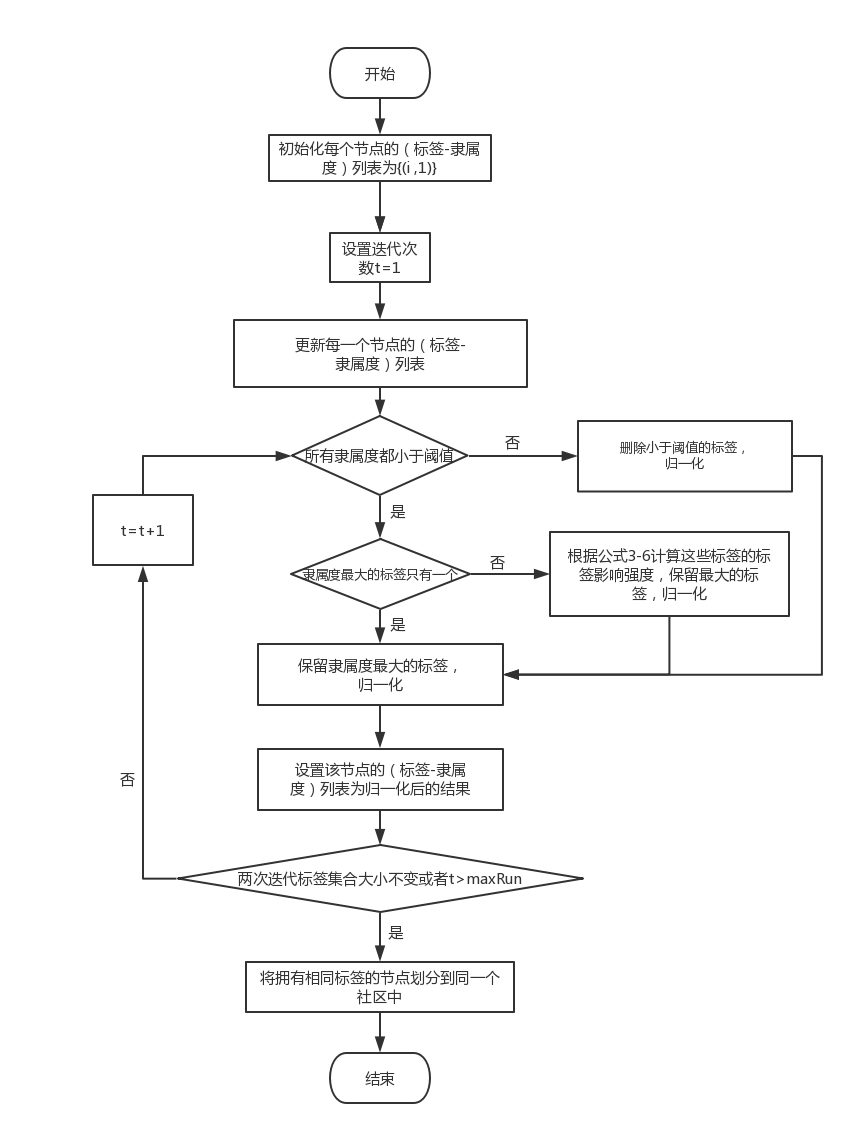
\includegraphics[width=1\textwidth]{figures/fig4-1}
  \caption{OCDABSLP算法流程图}\label{fig:fig4-1}
\end{figure}

\subsection{时间复杂度分析}
OCDABSLP 算法的时间复杂度分析如下: 

(1)为每个节点初始化标签所用时间复杂度为$ O(|V|)$; 

(2)每次标签传播过程分为两部分: 传统的标签传播过程:$O(v|E|log(v|E|/|V|))$;当节点属于所有社区的隶属度都小于阈值且最大值有多个时,利用
公式\ref{eqn:LI2}计算标签影响值的过程:$O(v|E|log(v|E|/|V|))$; 

(3)将相同标签的节点划分到一个社区的时间复杂度为 $O(|V|)$。 

标签传播过程是不断迭代执行的,因此整个算法的时间复杂度为
$2O(|V|)+2tO(v|E|log(v|E|/|V|))$。

% \section{算法伪代码}

\section{CDABSLP算法验证实验}
本节为本章提出的基于稳定标签传播的非重叠社区发现算法CDABSLP算法进行实验验证。首先介绍实验的软硬件环境和采用的数据集,然后对算法的评价指标进行简单阐述,最后是相关对比实验的结果展示与分析。

\subsection{实验环境}
本文实现的CDABSLP算法所使用的机器配置如表\ref{tab:tab3-1}所示。CDABSLP算法使用Python语言编程实现,均基于Python的复杂网络相关软件包Networkx,使用Anaconda来对软件包进行管理和部署,具体配置如表\ref{tab:tab3-2}所示。

\begin{table}
  \centering
  \caption{计算机硬件配置} \label{tab:tab3-1}
  \begin{tabular*}{0.9\textwidth}{@{\extracolsep{\fill}}cccc}
  \toprule
    处理器			&2.2GHz 双核 Intel Core i7 \\
    内存容量			&8 GB 1600 MHz DDR3 \\
    硬盘容量			&128GB 固态硬盘 \\
  \bottomrule
  \end{tabular*}
\end{table}

\begin{table}
  \centering
  \caption{计算机软件配置} \label{tab:tab3-2}
  \begin{tabular*}{0.9\textwidth}{@{\extracolsep{\fill}}cccc}
  \toprule
    操作系统			&macOS Sierra 10.12.6\\
    Anaconda版本  &conda 4.3.30 \\
    Networkx版本	&2.1 \\
    Python版本    &2.7.14\\
    Matplotlib版本  &2.0.2\\
    Numpy版本     &1.13.1\\
  \bottomrule
  \end{tabular*}
\end{table}

\subsection{数据集}
选用5个不同的真实数据集和LFR基准网络人工生成数据集进行实验验证本章所提算法的有效性。 

(1)真实数据集

在5个常用的真实网络数据集上进行实验验证本章算法的有效性,这5个真
实网络数据集包括Karate、Dolphins 和 Football 等,各个数据集的详细信息如表\ref{tab:tab3-3}所示;

Karate是 Zachary 空手道俱乐部成员关系网络,网络中的所有节点对应各个成员,边表示两个端点对应的成员是好朋友。网络包含 34 个节点,78 条边和两个社区。 

Dolphins是 Lusseau 等人对栖息在新西兰 Doubtful Sound 峡湾的一
个宽吻海豚群体进行长达 7 年的观察所构造出的海豚关系网,该群体包含 2 个家族共 62 只宽吻海豚。由这个群里的所有成员及它们间的接触关系构成一个包含
62 个节点,159 条边和两个社区的网络。

Polbooks是从 Amazon 的图书销售记录抽象得到的网络数据集,
分析了 105 本与美国政治相关的书和它们的 441 条共同销售关系,依据亚马逊上
对图书的观点和评价情况,将这些书分为“自由派”、“中间派”和“保守派”三
个类。因此,此数据集包含 105 个节点,441 条边和三个社区。

Football是分析美国高校橄榄球比赛对阵表得到的数据集。共有 115
所高校派出代表队参赛,共进行了 616 场比赛,按各代表队地区的不同将这个包
含 115 个节点 616 条边的网络分为 12 个社区。 

Email是由 Guimer 等人收集公布的,包含位于西班牙加泰罗尼亚
自治区的罗维拉-威尔吉利大学(简称 URV)的教师和研究生之间的邮件往来关
系。两个用户或者说两个邮箱地址如果互相发送过邮件,就构成一条边。网络包
含 1133 个节点和 5451 条边。

\begin{table}
  \centering
  \caption{真实网络数据集} \label{tab:tab3-3}
  \begin{tabular*}{0.9\textwidth}{@{\extracolsep{\fill}}cccc}
  \toprule
    数据集名称		&节点数   &边数   &社区数\\
  \midrule
    Karate  &34 &78 &2\\
    Dolphins	&62 &159  &2\\
    Polbooks  &105  &441  &3\\
    Football  &115  &616  &12\\
    Email     &1133 &5451 \\
  \bottomrule
  \end{tabular*}
\end{table}

(2)LFR人工基准网络

LFR基准网络是目前在社区发现领域使用最多的人工数据集之一。通
过调整网络生成参数可以产生用户需要的不同的人工数据集,LFR 基准网络的主
要生成参数及其含义如表\ref{tab:tab3-4}所示。

\begin{table}
  \centering
  \caption{LFR基准网络生成参数及其含义} \label{tab:tab3-4}
  \begin{tabular*}{0.9\textwidth}{@{\extracolsep{\fill}}cccc}
  \toprule
    参数		&含义\\
  \midrule
    N  &节点数\\
    avgk	&节点平均度\\ 
    maxk  &节点最大度\\
    mu  &网络拓扑结构混合参数\\
    minc  &最小社区规模\\
    maxc  &最大社区规模 \\
    on    &重叠节点个数\\
    om    &重叠节点可属于的社区个数\\
  \bottomrule
  \end{tabular*}
\end{table}

在 LFR 模型众多的生成参数中,混合参数$ mu \in [0,1]$是非常重要的一个参数,
mu 越小,说明连接社区之间的边越少,社区之间越“分离”,社区划分的难度随
着 mu 的增长而增大。on 和 om 两个参数用于生成具有重叠社区的数据集,生成
具有非重叠社区结构的数据集时,只需将 on 设置为 0,om 设置为 1 即可。 
生成六组具有非重叠社区结构的 LFR 基准网络数据集,所有的网络共享的
相同参数是 maxk = 50、on = 0 和 om = 1。每组包含九个 mu 值不同的数据集,分
别为 0.1 到 0.9,每组中的九个数据集共享参数 N、avgk、minc 和 maxc。其他参
数都取默认值。表\ref{tab:tab3-5}展示了这六组网络详细的生成参数情况。 

\begin{table}
  \centering
  \caption{六组LFR基准网络生成参数} \label{tab:tab3-5}
  \begin{tabular*}{0.9\textwidth}{@{\extracolsep{\fill}}ccccccc}
  \toprule
    编号		&N  &avgk &maxk &minc &maxc &mu\\
  \midrule
    1	&1000  &10 &50 &10 &50 &$0.1\sim 0.9$\\
    2 &1000  &10 &50 &20 &100 &$0.1\sim 0.9$\\
    3 &5000  &10 &50 &10 &50 &$0.1\sim 0.9$\\
    4 &5000  &10 &50 &20 &100 &$0.1\sim 0.9$\\
    5 &1000  &20 &50 &10 &50 &$0.1\sim 0.9$\\
    6 &1000  &20 &50 &20 &100 &$0.1\sim 0.9$\\
  \bottomrule
  \end{tabular*}
\end{table}

\subsection{评价指标}
迄今为止,出现了各种各样的社区发现算法,如何评价不同的的发现算法的好坏是一个非常重要的问题。为此,学者们提出了多种社区结构评价指标用来评价网络社区划分质量,其中比较有代表性的有模块度、NMI。下面介绍这些指标。

(1)模块度

模块度是目前学者们最常用和经典的网络社区结构评价指标,它最初是被Newman等人于2004年提出来的\cite{2002Community}。其通过比较现有网络和基准网络在相同社区划分下的连接密度差来衡量网络社区的优劣,其中基准网络是由原网络具有相同度序列的随机网络。模块度计算方式详见公式\ref{eqn:modular}。

\begin{equation}
  \label{eqn:modular}
  Q=\frac{1}{2m}\sum_{i,j}\left [ A_{ij}-\frac{k_ik_j}{2m} \right ]\delta (c_i, c_j)  
\end{equation}

其中,A 表示网络中的邻接矩阵, m 表示网络中边的总数,$k_i$和$k_j$表示节点 i 和 j 的度数,$c_i$和$c_j$表示节点 i 和 j 所属的社区。如果$i=j,\delta(c_i,c_j)=1$,反之$\delta(c_i,c_j)=0$

(2)NMI

随着在线社交网络的发展,人们发现在线社交网络的很多数据中存在着暗示各个节点的社区属性信息。例如,在人人网的学校信息便揭示了网络节点中属于同一学校的社区结构,Facebook中的兴趣信息同样表征了具有相同兴趣的虚拟用户群体。这些数据在为社区发现问题提供了丰富的信息的同时,也在一定程度上为虚拟社区结构优劣的评判提供了标准答案。针对这种预先拥有一定虚拟社区结构信息的情况下,Leon Danon等人[34]提出了Normalized Mutual Information(NMI)利用信息化熵来衡量算法划分的社区结构和预先已知的社区结构之间的差异。NMI是基于混合矩阵(Confusion Matrix)N来计算的数字指标。NMI计算方式详见公式\ref{eqn:nmi}。

\begin{equation}
  \label{eqn:nmi}
  NMI=\frac{ -2 \sum_{i,j} N_{ij}  ln{\frac{N_{ij}}{N_iN_j}} } {\sum_{i}N_iln{\frac{N_i}{n}}+\sum_{j}N_jln{\frac{N_j}{n}}}
\end{equation}

使用该数字指标,可以衡量划分出来的社区结构与已知的网络社区结构的差异程度值,该值越大,则表明获得的社区结构划分越好,当该值达到最大化值1时,说明算法发现的社区结构与已知社区结构完全已知,效果最好。

\begin{figure}
 \centering
 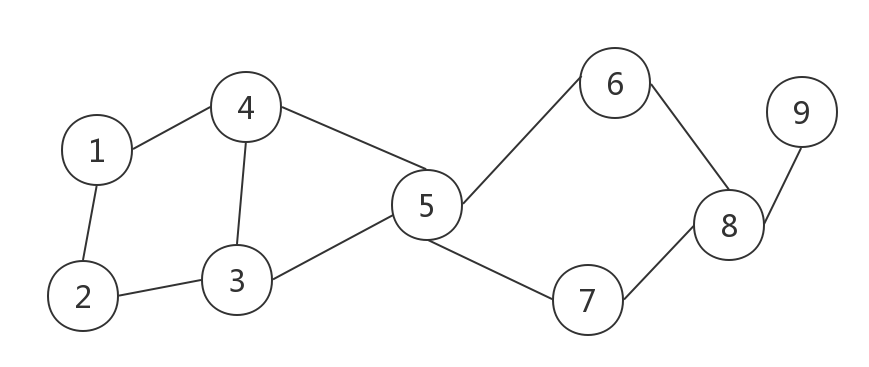
\includegraphics[width=0.75\textwidth]{figures/fig5-1}
 \caption{NMI网络示例图}\label{fig:fig5-1}
\end{figure}

下面以图\ref{fig:fig5-1}为例来说明计算NMI的过程。假设已知的最佳社区结构划分为集合{1,2,3,4}和{5,6,7,8},相应的社区划分向量表示为a = (1,1,1,1,2,3,3,3,3),再假设某算法获得的社区划分结构可以用向量表示为b = (3,3,3,3,2,1,1,1,1)来表示。根据已知的社区划分向量,可以构造混合矩阵\ref{eqn:n}。

\begin{equation}
  \label{eqn:n}
  N=\begin{bmatrix}
    0 & 0 &4 \\ 
    0 & 1 & 0\\ 
    4 & 0 & 0
    \end{bmatrix}
\end{equation}

根据上式计算可知,该划分的NMI值为1。

\subsection{对比实验}
